\documentclass[a4paper,12pt]{article}
\usepackage[UTF8]{ctex}
\usepackage{graphicx}

\graphicspath{{figures/}}
\begin{document}

% \setcounter{page}{0}
% \thispagestyle{empty}
% \tableofcontents
% \setcounter{page}{0}
% \thispagestyle{empty}
% \newpage
% \setcounter{page}{1}

% 章节内容如下

% 插图原代码,优先使用内置的latex语法,其次使用inkspace生成的svg->eps图片
\section{Welcome}

使用Latex写技术相关书籍。

$2x+3y=34$


$f(x, y) = 100 * \lbrace[(x + y) * 3] - 5\rbrace$

write algorithm with math format.


\section{chaper01}

chapter 001,
chapter 002,
details for chapter01


\section{这里还是描述各类架构的设计吧}
\subsection{1}

\subsection{1}

\subsection{1}

\subsection{1}

\subsection{1}


\section{Pandas details}

contents about pandas all put here!


\section{Figures here}
\begin{figure}
\centering
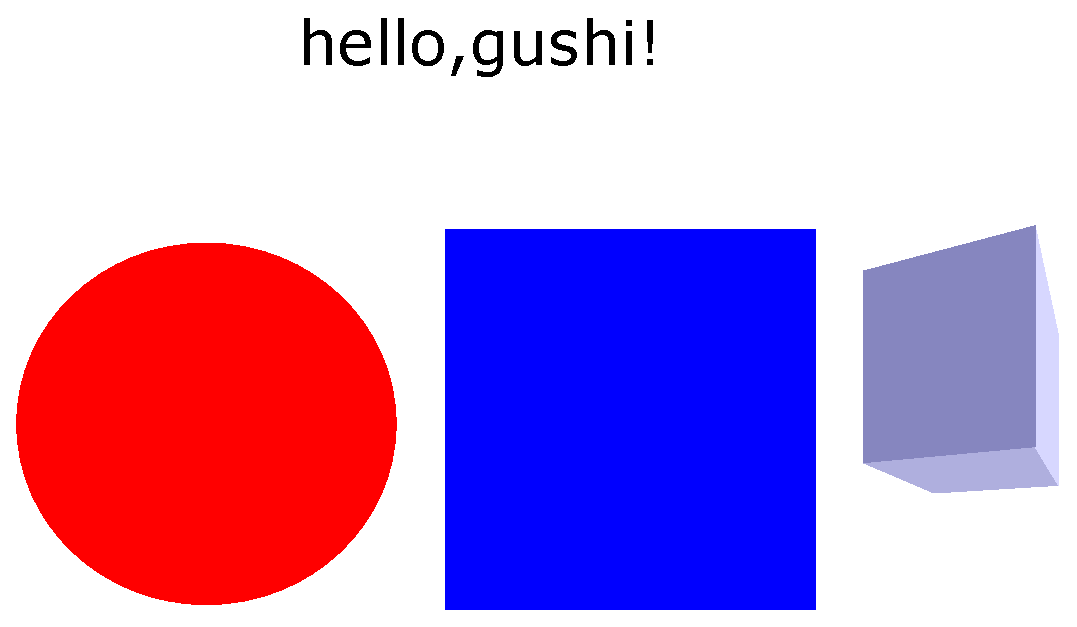
\includegraphics[width=\textwidth]{hello.eps}
\caption{title}
\end{figure}

\section{中文}

\section{Figures here}
\begin{figure}
\centering
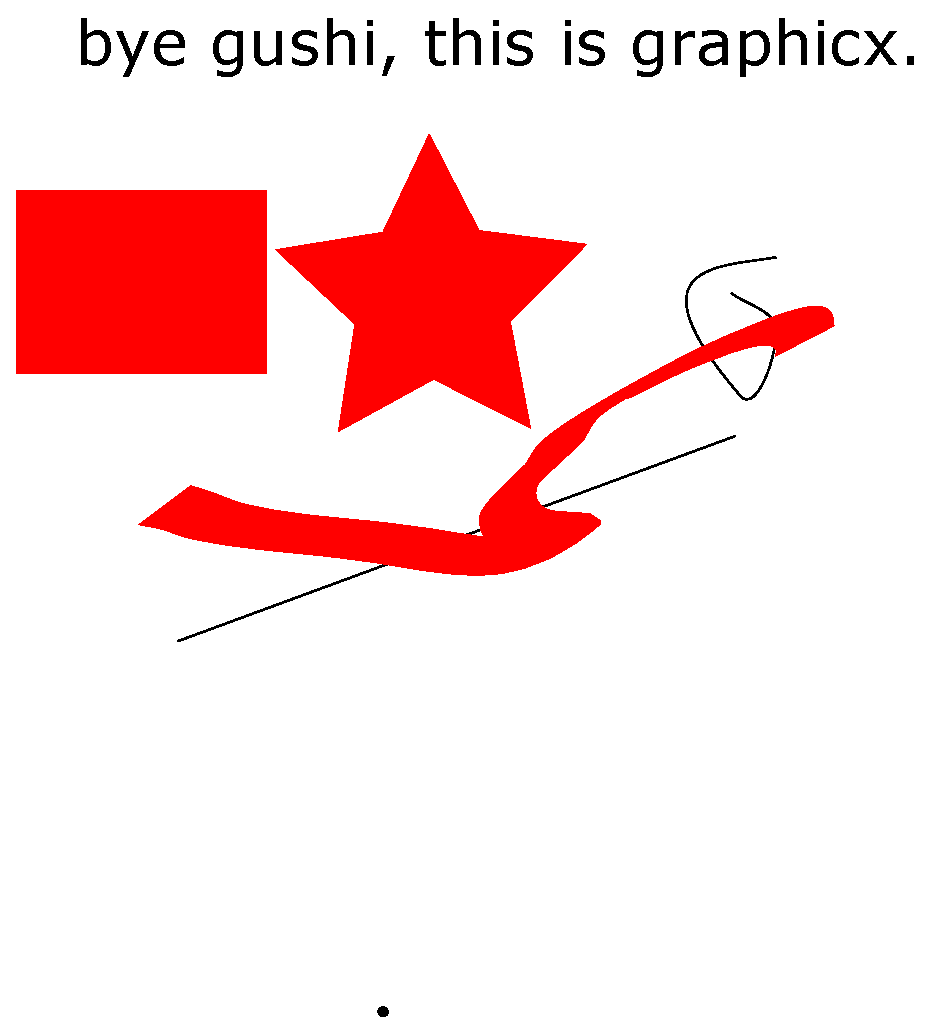
\includegraphics[width=\textwidth]{bye.eps}
\caption{title}
\end{figure}

\section{Bye}

\renewcommand\refname{}
\nocite{*}
\bibliographystyle{IEEEtran}
\bibliography{IEEEabrv,REFS}
\end{document}
